\documentclass[convert = false, tikz]{standalone}
\usepackage[utf8]{inputenc}
\usepackage{tikz}
\usetikzlibrary{automata, positioning, arrows}
 
\usepackage{../../../../style_automata}

% arara: pdflatex
% arara: latexmk: { clean: partial }
\begin{document}
    \tikzset{
    node distance=2.5cm, % specifies the minimum distance between two nodes.
    }
    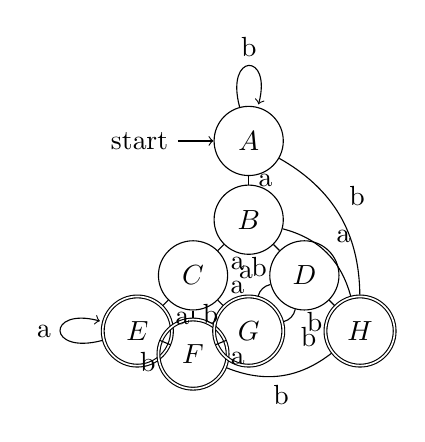
\begin{tikzpicture}
        \node[state, initial] (a) {$A$};
        \node[state, below of=a] (b) {$B$};
        \node[state, below left of=b] (c) {$C$};
        \node[state, below right of=b] (d) {$D$};
        \node[state, accepting, below left of=c] (e) {$E$};
        \node[state, accepting, below of=c] (f) {$F$};
        \node[state, accepting, below right of=c] (g) {$G$};
        \node[state, accepting, below right of=d] (h) {$H$};
        \draw (a) edge[loop above] node{b} (a)
        (a) edge[right] node{a} (b)
        (b) edge[below right] node{a} (c)
        (b) edge[below left] node{b} (d)
        (c) edge[below right] node{a} (e)
        (c) edge[right] node{b} (f)
        (d) edge[above left, bend right=30] node{a} (g)
        (d) edge[below left] node{b} (h)
        (e) edge[loop left] node{a} (e)
        (e) edge[below left] node{b} (f)
        (f) edge[below right] node{a} (g)
        (f) edge[below, bend right=30] node{b} (h)
        (g) edge[above right] node{a} (c)
        (g) edge[below right, bend right=30] node{b} (d)
        (h) edge[above right, bend right=30] node{b} (a)
        (h) edge[above right, bend right=30] node{a} (b)
        ;
    \end{tikzpicture}
\end{document}
